\let\negmedspace\undefined
\let\negthickspace\undefined
\documentclass[journal]{IEEEtran}
\usepackage[a5paper, margin=10mm, onecolumn]{geometry}
\usepackage{lmodern} % Ensure lmodern is loaded for pdflatex
\usepackage{tfrupee} % Include tfrupee package

\setlength{\headheight}{1cm} % Set the height of the header box
\setlength{\headsep}{0mm}  % Set the distance between the header box and the top of the text
\usepackage{romannum}
\usepackage{csquotes}
\usepackage{gvv-book}
\usepackage{gvv}
\usepackage{circuitikz}
\usepackage{cite}
\usepackage{float}
\usepackage{amsmath,amssymb,amsfonts,amsthm}
\usepackage{algorithmic}
\usepackage{graphicx}
\usepackage{textcomp}
\usepackage{xcolor}
\usepackage{txfonts}
\usepackage{listings}
\usepackage{enumitem}
\usepackage{mathtools}
\usepackage{gensymb}
\usepackage{comment}
\usepackage[breaklinks=true]{hyperref}
\usepackage{tkz-euclide} 
\usepackage{listings}
% \usepackage{gvv}                                        
\def\inputGnumericTable{}                                 
\usepackage[latin1]{inputenc}                                
\usepackage{color}                                            
\usepackage{array}                                            
\usepackage{longtable}                                       
\usepackage{calc}                                             
\usepackage{multirow} 
\usepackage{multicol}
\usepackage{hhline}   
\usepackage{enumitem}
\usepackage{ifthen}                                           
\usepackage{lscape}
\usepackage{caption}
\usepackage{tikz}
\usetikzlibrary{patterns}

\title{GATE 2017 Question Paper (Life Sciences - XL)}
\author{EE25BTECH11019 \\ Vivek Darji}
\date{}

\begin{document}

\maketitle
\section*{Chemistry (XL-P)}
\setcounter{enumi}{0}
\begin{enumerate}

\item CO reacts readily with\hfill $\brak{\text{GATE XL 2017}}$
\begin{enumerate}
\begin{multicols}{4}
    \item Fe
    \item Fe$^{2+}$
    \item Fe$^{3+}$
    \item Fe$^{4+}$
\end{multicols}
\end{enumerate}

\item Molecules that are NOT isoelectronic to NO$^+$ ion are\hfill $\brak{\text{GATE XL 2017}}$
\begin{enumerate}
\begin{multicols}{2}
    \item CO$^+$ and N$_2$
    \item NCO and H$_3$BCN
    \item BO$_2^-$ and H$_3$C--C$\equiv$CH
    \item OF$_2$ and O$_3^+$
\end{multicols}
\end{enumerate}

\item The extensive quantity among the following is\hfill $\brak{\text{GATE XL 2017}}$
\begin{enumerate}
\begin{multicols}{2}
    \item Pressure
    \item Temperature
    \item Chemical potential
    \item Volume
\end{multicols}
\end{enumerate}

\item The compound that gives characteristic foul smell upon heating with potassium hydroxide and chloroform is\hfill $\brak{\text{GATE XL 2017}}$
\begin{figure}[H]
    \centering
    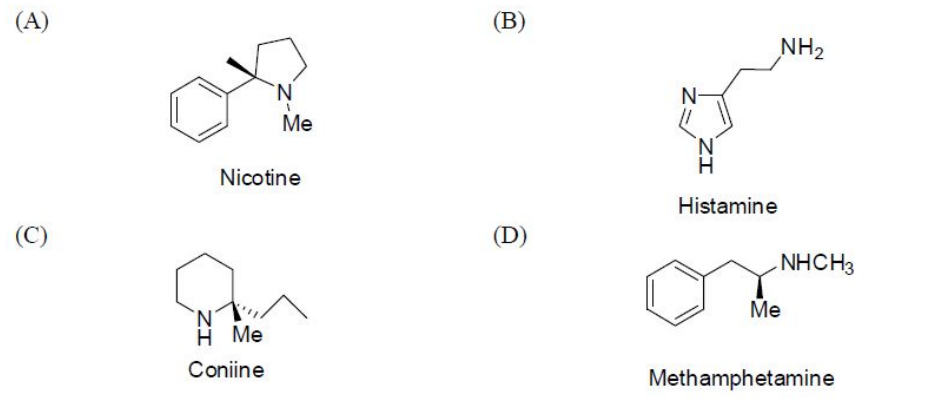
\includegraphics[width=0.8\columnwidth]{figs/xl2017_q4_all_opts.png}
    \caption{Q4 options}
\end{figure}

\item The correct order of stability in water is\hfill $\brak{\text{GATE XL 2017}}$
\begin{figure}[H]
    \centering
    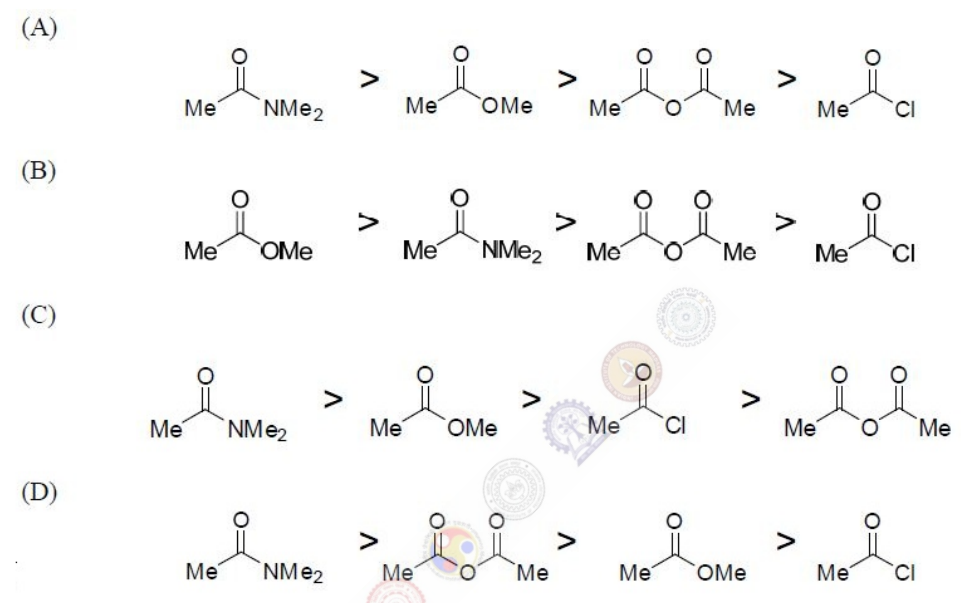
\includegraphics[width=0.8\columnwidth]{figs/xl2017_q5_all_opts.png}
    \caption{Q5 options}
\end{figure}

\item The pair of molecules having non-linear structures is\hfill $\brak{\text{GATE XL 2017}}$
\begin{enumerate}
\begin{multicols}{4}
    \item ICl$_3$ and BeH$_2$
    \item CS$_2$ and I$_3^-$
    \item SO$_3$ and ClO$_2^-$
    \item XeF$_2$ and CN$^-$
\end{multicols}
\end{enumerate}

\item The decreasing order of bond lengths for O$_2$, B$_2$, N$_2$ and C$_2$ is\hfill $\brak{\text{GATE XL 2017}}$
\begin{enumerate}
\begin{multicols}{2}
    \item B$_2$ $>$ C$_2$ $>$ N$_2$ $>$ O$_2$
    \item B$_2$ $>$ C$_2$ $>$ O$_2$ $>$ N$_2$
    \item N$_2$ $>$ C$_2$ $>$ O$_2$ $>$ B$_2$
    \item B$_2$ $>$ O$_2$ $>$ N$_2$ $>$ C$_2$
\end{multicols}
\end{enumerate}

\item The octahedral metal oxide with the highest CFSE value is\hfill $\brak{\text{GATE XL 2017}}$
\begin{enumerate}
\begin{multicols}{4}
    \item ZnO
    \item MnO
    \item VO
    \item TiO
\end{multicols}
\end{enumerate}

\item Assuming independent non-interacting electrons, the first ionization energy of Helium atom is\hfill $\brak{\text{GATE XL 2017}}$
\begin{enumerate}
\begin{multicols}{4}
    \item $13.6$ eV
    \item $27.2$ eV
    \item $54.4$ eV
    \item $108.8$ eV
\end{multicols}
\end{enumerate}

\item For a reaction A + B $\longrightarrow$ products, the following data was obtained:  
$[A]_0$ and $[B]_0$ are initial concentrations of A and B, respectively. The overall order of the reaction is\hfill $\brak{\text{GATE XL 2017}}$
\begin{enumerate}
\begin{multicols}{4}
    \item 2
    \item 3
    \item 4
    \item 5
\end{multicols}
\end{enumerate}
\item The EMF for the following cell at $298.15\ \mathrm{K}$ is\hfill $\brak{\text{GATE XL 2017}}$\\
Ag(s) $\mid$ Ag$^{+}$(aq., 0.01 M) $\parallel$ Ag$^{+}$(aq., 1.0 M) $\mid$ Ag(s)\\
(Standard reduction potential for Ag$^{+}$ + e$^{-} \rightarrow$ Ag is $-0.80$ V)
\begin{enumerate}
\begin{multicols}{4}
    \item 0.12 V
    \item 0.68 V
    \item 0.80 V
    \item 0.92 V
\end{multicols}
\end{enumerate}

\item One gram of a protein is dissolved in one liter of water. The resulting solution exerts an osmotic pressure of $1.4$ Torr at $298\ \mathrm{K}$. Assuming that the protein does not ionize in solution, the molecular weight of the protein is  \underline{\rule{2cm}{0pt}} g mol$^{-1}$. (R = $0.082\ \mathrm{L\ atm\ mol^{-1}\ K^{-1}}$)\hfill $\brak{\text{GATE XL 2017}}$

\item The type of nucleophilic substitution and the possible products for each of the reactions P and Q are\hfill $\brak{\text{GATE XL 2017}}$
\begin{figure}[H]
    \centering
    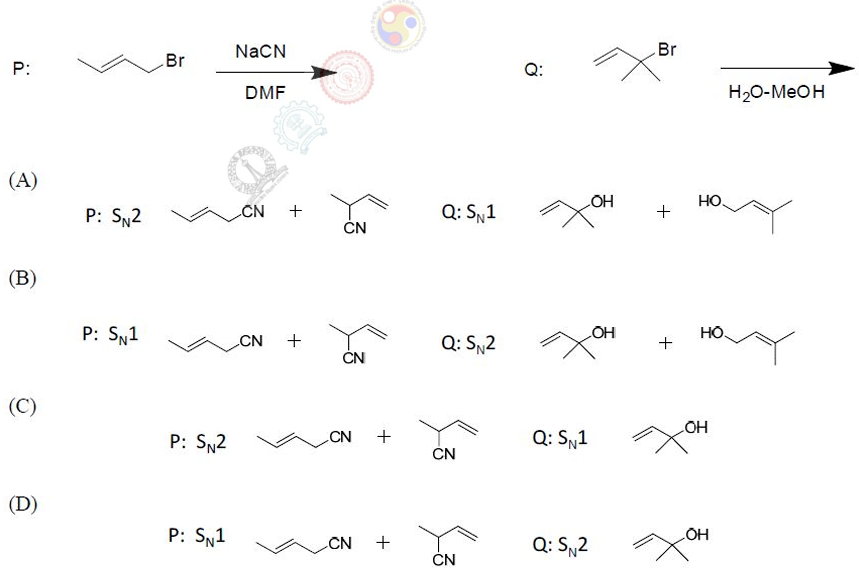
\includegraphics[width=0.85\columnwidth]{figs/xl2017_q13_all_opts.png}
    \caption{Q13 options}
\end{figure}

\item If mono-chlorination occurs at every carbon in the following reaction, the number of isomers (stereo isomers + constitutional isomers) that one can have is\hfill $\brak{\text{GATE XL 2017}}$
\begin{figure}[H]
    \centering
    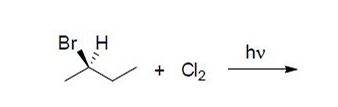
\includegraphics[width=0.65\columnwidth]{figs/xl2017_q14.png}
    \label{fig:placeholder}
    \caption{Q14 options}
\end{figure}
\begin{enumerate}
\begin{multicols}{4}
    \item 4
    \item 5
    \item 6
    \item 8
\end{multicols}
\end{enumerate}

\item The major product in the following reaction is\hfill $\brak{\text{GATE XL 2017}}$
\begin{figure}[H]
    \centering
    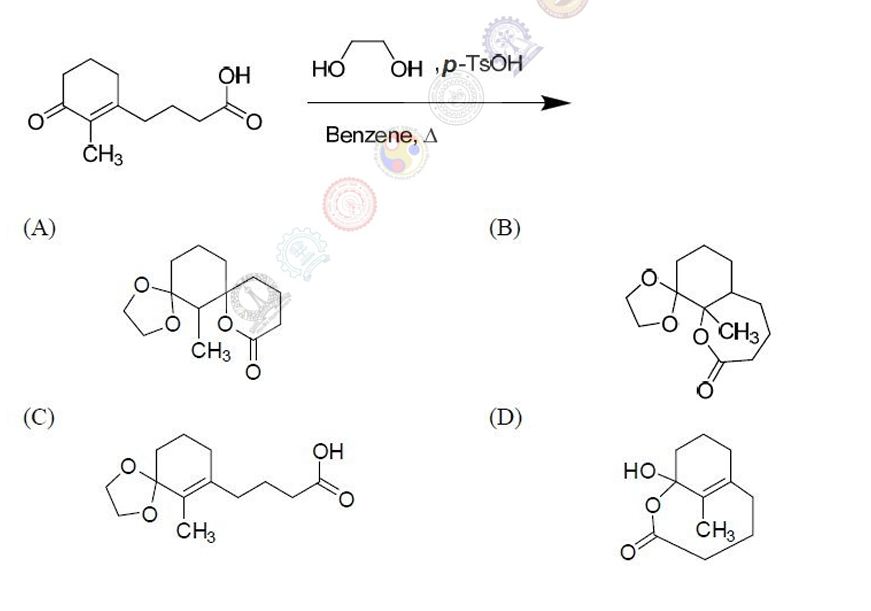
\includegraphics[width=0.85\columnwidth]{figs/xl2017_q15_all_opts.png}
    \caption{Q15}
    \label{fig:placeholder}
\end{figure}

\section*{Biochemistry (XL-Q)}
\setcounter{enumi}{15}

\item The molecular weight of a protein as determined by native PAGE is $400\ \mathrm{kDa}$. This protein when run on a non-reducing SDS-PAGE gave a band of $200\ \mathrm{kDa}$, and on a reducing SDS-PAGE, gave a band of $100\ \mathrm{kDa}$. The protein has\hfill $\brak{\text{GATE XL 2017}}$
\begin{enumerate}
    \item Four subunits of which two sets are linked by two disulfide bridges
    \item Four subunits which are linked by four disulfide bridges
    \item Two subunits only and none are linked by disulfide bridges
    \item Two subunits which are linked by disulfide bridges
\end{enumerate}

\item Which one of the following techniques CANNOT be used to determine the sequence of a novel protein?\hfill $\brak{\text{GATE XL 2017}}$
\begin{enumerate}
    \item De novo sequencing by ESI-MS/MS
    \item Edman degradation
    \item Sanger sequencing
    \item Peptide mass fingerprinting
\end{enumerate}

\item Which type of polyacrylamide gel can be used for analyzing the four different proteins listed below?\\
Protein P: $60\ \mathrm{kDa}$, pH 4\\
Protein Q: $45\ \mathrm{kDa}$, pH 8\\
Protein R: $60\ \mathrm{kDa}$, pH 6\\
Protein S: $45\ \mathrm{kDa}$, pH 7.5\hfill $\brak{\text{GATE XL 2017}}$
\begin{enumerate}
    \item 20\% gel, pH 4--7
    \item 20\% gel, pH 3--10
    \item 12\% gel, pH 3--10
    \item 12\% gel, pH 4--7
\end{enumerate}

\item The number of fragments generated when the peptide `ANDCQEGKFMLKPDTWRYVSFMRPA` is subjected to complete digestion with trypsin are  \underline{\rule{2cm}{0pt}}\hfill $\brak{\text{GATE XL 2017}}$

\item Puromycin is a structural analog of\hfill $\brak{\text{GATE XL 2017}}$
\begin{enumerate}
\begin{multicols}{4}
    \item alanyl-tRNA
    \item tyrosyl-tRNA
    \item methionyl-tRNA
    \item glycyl-tRNA
\end{multicols}
\end{enumerate}

\item Which one of the enzymes is responsible for arsenic toxicity?\hfill $\brak{\text{GATE XL 2017}}$
\begin{enumerate}
\begin{multicols}{2}
    \item Pyruvate kinase
    \item Aldolase
    \item Phosphofructokinase
    \item Pyruvate dehydrogenase
\end{multicols}
\end{enumerate}

\item Which one is TRUE for Calvin cycle?\hfill $\brak{\text{GATE XL 2017}}$
\begin{enumerate}
    \item Glycerol 3-phosphate is generated in this cycle
    \item CO$_2$ is not consumed in this cycle
    \item This is a reductive pentose phosphate cycle
    \item Ribose 5-phosphate is a carboxylation substrate in this cycle
\end{enumerate}

\item Administration of primaquine causes severe hemolytic anemia because it\hfill $\brak{\text{GATE XL 2017}}$
\begin{enumerate}
    \item Increases the demand for NADPH to a level that cells $ \text{can't} $ meet
    \item Decreases the demand for NADPH
    \item Inactivates glutathione peroxidase of erythrocytes
    \item Increases reduced glutathione level of erythrocytes
\end{enumerate}

\item Which one of the following will NOT form lipid bilayer?\hfill $\brak{\text{GATE XL 2017}}$
\begin{multicols}{2}
\begin{enumerate}
\item Cholesterol
\item Phosphatidyl ethanolamine
\item Triacylglycerol
\item Phosphatidyl serine
\end{enumerate}
\end{multicols}

\item Which one of the following features is NOT appropriate for Fab fragment of IgG?\hfill $\brak{\text{GATE XL 2017}}$
\begin{enumerate}
\item Contains antigen binding site
\item Contains an intact L chain
\item Two fragments are formed from one IgG molecule
\item Mediates complement fixation in the intact IgG molecule
\end{enumerate}

\item The duration of DNA synthesis \brak{S phase} in plant cells is $11 \ \mathrm{h}$ and the DNA is replicated at a rate of $100 \ \mathrm{bp/fork}$. A plant species has about $3.0\times 10^{10} \ \mathrm{bp/genome}$. The number of bidirectional forks per genome required for replication will be \underline{\rule{2cm}{0pt}}.\hfill $\brak{\text{GATE XL 2017}}$

\item In a PCR reaction, with one double stranded DNA of $600 \ \mathrm{bp}$, nano gram of DNA produced after $40$ cycles of amplification will be\underline{\rule{2cm}{0pt}}.\hfill $\brak{\text{GATE XL 2017}}$

\item A solution containing GTP has molar extinction coefficient of $1.55\times 10^{4} \ \mathrm{mol^{-1} dm^{3} cm^{-1}}$ at a given wavelength. The concentration of GTP solution is $1.290\times 10^{-5} \ \mathrm{mol \ dm^{-3}}$. The absorbance of GTP solution in $1 \ \mathrm{cm}$ cuvette at the same wavelength will be \underline{\rule{2cm}{0pt}}.\hfill $\brak{\text{GATE XL 2017}}$

\item Which one of the following is NOT TRUE for class I MHC protein?\hfill $\brak{\text{GATE XL 2017}}$
\begin{enumerate}
\item MHC class I protein are polymorphic
\item T-cell receptors recognizes MHC class I protein
\item MHC class I protein are displayed on the surfaces of nucleated vertebrate cells
\item $\beta_{2}$-microglobulin is covalently associated with MHC class I protein
\end{enumerate}

\item In an enzyme catalyzed reaction, the initial reaction velocity is only one fourth of its maximum velocity. If the substrate concentration is $3.0\times 10^{-3} \ \mathrm{mM}$, the value of $K_m$ in micro molar \brak{\mu\mathrm{M}} will be \underline{\rule{2cm}{0pt}}\hfill $\brak{\text{GATE XL 2017}}$

\item Match the following enzymes in column I with their cofactors in column II:\hfill $\brak{\text{GATE XL 2017}}$
\begin{multicols}{2}
\noindent Column I  \\
P) Pyruvate decarboxylase \\
Q) Glyceraldehyde 3-phosphate dehydrogenase \\
R) Pyruvate carboxylase \\
S) Glucose-6-phosphate dehydrogenase  

\columnbreak

\noindent Column II \\ 
i. Biocytin \\
ii. NADP$^{+}$ \\
iii. NAD$^{+}$ \\
iv. Thiamine pyrophosphate
\end{multicols}
\begin{enumerate}
\item P-ii; Q-i; R-iv; S-iii
\item P-iv; Q-iii; R-i; S-ii
\item P-i; Q-ii; R-iii; S-iv
\item P-iii; Q-i; R-iv; S-ii
\end{enumerate}

\item Match the molecule in column I with its function in column II:\hfill $\brak{\text{GATE XL 2017}}$
\begin{multicols}{2}
\noindent Column I  \\
P) Cholera toxin \\
Q) Pertussis toxin \\
R) IP$_3$ \\
S) Caffeine  

\columnbreak

\noindent Column II  \\
i. modifies $G_{\alpha i}$ \\
ii. inhibits c-AMP phosphodiesterase \\
iii. modifies $G_{\alpha s}$ \\
iv. increases intracellular Ca$^{2+}$ level
\end{multicols}
\begin{enumerate}
\item P-iii; Q-i; R-iv; S-ii
\item P-iv; Q-i; R-iii; S-ii
\item P-ii; Q-iv; R-i; S-iii
\item P-iii; Q-i; R-ii; S-iv
\end{enumerate}

\item In an in vitro dehydrogenation reaction of succinate catalyzed by succinate dehydrogenase, malonate is added. Which one of the following curves represents the effect of malonate on the catalysis of succinate dehydrogenase?\hfill $\brak{\text{GATE XL 2017}}$
\begin{figure}[H]
    \centering
    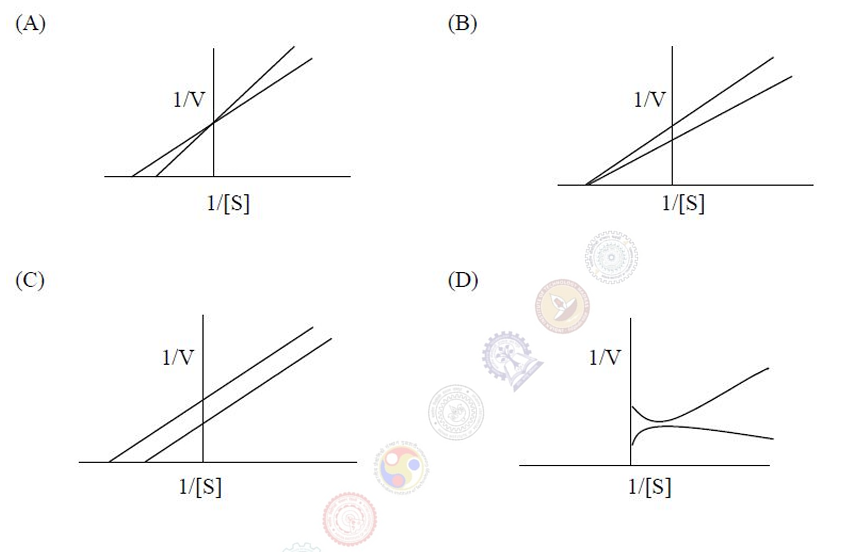
\includegraphics[width=0.9\columnwidth]{figs/q33_combined.png}
    \caption{Que. 33}
    \label{fig:placeholder}
\end{figure}

\item Cardiotonic steroids have ability to strengthen heart muscle contraction due to the fact that these steroids\hfill $\brak{\text{GATE XL 2017}}$
\begin{enumerate}
\item inhibit K$^{+}$-dependent dephosphorylation of Na$^{+}$-K$^{+}$ ATPase
\item activate Na$^{+}$-K$^{+}$ ATPase
\item increase uptake of Na$^{+}$ by activation of Na$^{+}$-Ca$^{2+}$ exchanger
\item increase uptake of Ca$^{2+}$ by activation of Na$^{+}$-Ca$^{2+}$ exchanger
\end{enumerate}

\item A newly isolated circular plasmid gave two bands of $3.2$ and $3$ kb on digestion with EcoRI and two bands of $5.0$ kb and $1.2$ kb on digestion with BamHI. Double digestion with EcoRI and BamHI, yielded four bands of $2.6$ kb, $2.4$ kb, $0.8$ kb and $0.4$ kb. Digestion with SalI led to disruption of ampicillin resistance gene cassette. The correct restriction map is\hfill $\brak{\text{GATE XL 2017}}$
\begin{figure}[H]
    \centering
    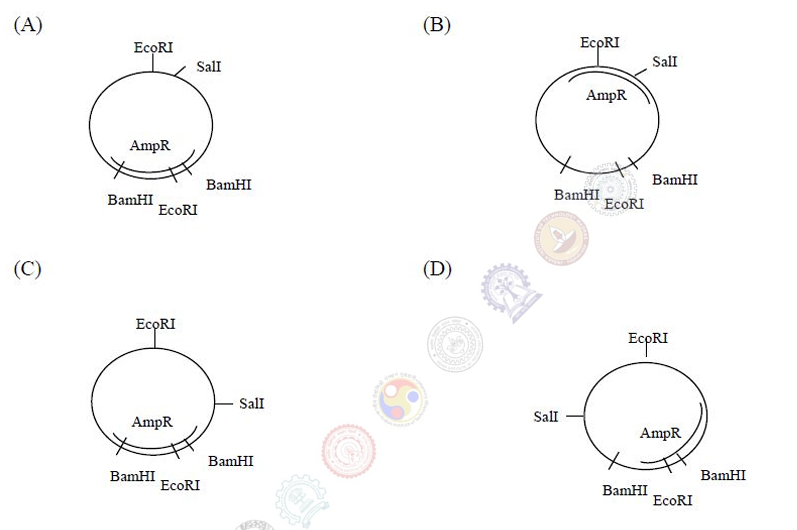
\includegraphics[width=0.9\columnwidth]{figs/q35_combined.png}
    \caption{Que. 35}
    \label{fig:placeholder}
\end{figure}

\section*{Botany (XL-R)}
\setcounter{enumi}{35}

\item As per the Angiosperm Phylogeny Group \brak{APG II, 2003} classification, which of the following plant families comprises of only single genus with single species?\hfill $\brak{\text{GATE XL 2017}}$
\begin{multicols}{2}
\begin{enumerate}
\item Lauraceae
\item Aristolochiaceae
\item Amborellaceae
\item Typhaceae
\end{enumerate}
\end{multicols}

\item A cavity, lysigenous in origin and possessing volatile oil is found in the pericarp of one of the following plants. Identify the CORRECT answer.\hfill $\brak{\text{GATE XL 2017}}$
\begin{multicols}{4}
\begin{enumerate}
\item Litchi
\item Citrus
\item Mango
\item Coconut
\end{enumerate}
\end{multicols}

\item Among the following, which genetic material is naturally inherited through maternal inheritance in higher plants?\hfill $\brak{\text{GATE XL 2017}}$
\begin{multicols}{2}
\begin{enumerate}
\item Nuclear DNA
\item Plasmid DNA
\item Chloroplast DNA
\item T-DNA
\end{enumerate}
\end{multicols}

\item A typical floral meristem differs from shoot apical meristem on the basis of\hfill $\brak{\text{GATE XL 2017}}$
\begin{multicols}{2}
\begin{enumerate}
\item Determinate growth
\item Presence of auxin
\item Presence of stem cells
\item Negative geotropism
\end{enumerate}
\end{multicols}

\item Which of the following plant hormones is a carotenoid-cleavage product? \hfill $\brak{\text{GATE XL 2017}}$
\begin{enumerate}
\begin{multicols}{2}
    \item Phytosulfokine
    \item Brassinosteroid
    \item Methyl jasmonate
    \item Strigolactone
\end{multicols}
\end{enumerate}

\item Two of the \textit{vir} operons of Ti plasmid in \textit{Agrobacterium tumefaciens} are constitutively expressed. Identify the CORRECT pair. \hfill $\brak{\text{GATE XL 2017}}$
\begin{enumerate}
    \item \textit{virA} and \textit{virG}
    \item \textit{virF} and \textit{virH}
    \item \textit{virC} and \textit{virD}
    \item \textit{virB} and \textit{virE}
\end{enumerate}

\item Which of the following fungi is an example of obligate biotrophic plant pathogen? \hfill $\brak{\text{GATE XL 2017}}$
\begin{enumerate}
\begin{multicols}{2}
    \item \textit{Alternaria brassicicola}
    \item \textit{Botrytis cinerea}
    \item \textit{Puccinia triticina}
    \item \textit{Sclerotinia sclerotiorum}
\end{multicols}
\end{enumerate}

\item The phenomenon where an organism lives at the expense of another organism by harming it but not killing, is called \hfill $\brak{\text{GATE XL 2017}}$
\begin{enumerate}
\begin{multicols}{4}
    \item Commensalism
    \item Predation
    \item Symbiosis
    \item Parasitism
\end{multicols}
\end{enumerate}

\item Which of the following is TRUE for $K$-strategist species? \hfill $\brak{\text{GATE XL 2017}}$
\begin{enumerate}
    \item Produce relatively large number of offspring
    \item Population often grow exponentially
    \item Provide relatively little or no parental care to offspring
    \item Occur in stable and predictable habitats
\end{enumerate}

\item Identify the INCORRECT statement with relation to plant secondary metabolites. \hfill $\brak{\text{GATE XL 2017}}$
\begin{enumerate}
    \item Atropine is a member of indole alkaloids
    \item Limonene is a cyclic terpene found in citrus plants
    \item Green tea is rich in polyphenols
    \item Cyanidin contributes to the red color in rose petals
\end{enumerate}

\item Choose the CORRECT set of matches between group I and group II in relation to nitrogen fixation and assimilation \hfill $\brak{\text{GATE XL 2017}}$

\begin{multicols}{2}
\noindent Column I  \\
P) Nitrobacter \\
Q) Nitrite reductase \\
R) Nitrogenase \\
S) Nitrate reductase 

\columnbreak

\noindent Column II \\ 
i. NO$_3^-$ $\to$ NO$_2^-$ \\
ii. N$_2$ $\to$ NH$_3$ \\
iii. NO$_2^-$ $\to$ NH$_4^+$ \\
iv. NO$_2^-$ $\to$ NO$_3^-$
\end{multicols}

\begin{enumerate}
    \item P-4, Q-3, R-2, S-1
    \item P-4, Q-3, R-1, S-2
    \item P-1, Q-2, R-4, S-3
    \item P-3, Q-4, R-2, S-1
\end{enumerate}

\item Two plant cells M and N are lying side by side making direct contact. ``M'' has osmotic potential $\Psi_s$ of $-10$ bar and pressure potential $\Psi_p$ of $4$ bar. On the other hand, ``N'' has osmotic potential $\Psi_s$ of $-12$ bar and pressure potential $\Psi_p$ of $5$ bar.\\
Based on these data, what would be the direction of movement of water between M and N? \hfill $\brak{\text{GATE XL 2017}}$
\begin{enumerate}
\begin{multicols}{2}
    \item M to N
    \item N to M
    \item There will be no movement
    \item In both directions
\end{multicols}
\end{enumerate}

\item Two independent non-segregating recessive mutants $\brak{m1 \text{ and } m2}$ display similar defects in petal formation. When they were crossed with each other $\brak{m1 \times m2}$, all the F$_1$ plants developed normal petals. In view of this observation, which of the following conclusions is CORRECT? \hfill $\brak{\text{GATE XL 2017}}$
\begin{enumerate}
    \item Mutations in both $m1$ and $m2$ are in the same gene
    \item Mutations in both $m1$ and $m2$ are in two separate genes
    \item Inheritance is non-Mendelian
    \item None of the above
\end{enumerate}

\item In a hypothetical trihybrid cross of three loci $\brak{\text{viz.\ } A,B,C}$, all were inherited in a complete dominant manner over their recessive alleles $a,b,c$, respectively. When a test cross between F$_1$ and parent ``$aabbcc$'' was performed, following genotypes of eight phenotypically distinct classes were observed with respective numbers \hfill $\brak{\text{GATE XL 2017}}$

\begin{center}
\begin{tabular}{ll}
    \textbf{Group I} & \textbf{Group II} \\
    P. Ferrite & 1. Hexagonal Close Packed (HCP) \\
    Q. Austenite & 2. Body Centered Cubic (BCC) \\
    R. Martensite & 3. Body Centered Tetragonal (BCT) \\
    & 4. Face Centered Cubic (FCC)
\end{tabular}
\end{center}

The genetic distance $\brak{\text{up to one decimal}}$ between $A$ and $C$ loci will be \underline{\rule{2cm}{0pt}} cM.

\item In a typical sexually reproducing angiospermic plant, if an endosperm cell contains $4.8\times10^8$ nucleotide pairs of DNA, then a microsporocyte of this plant will have \underline{\rule{2cm}{0pt}} $\times 10^8$ nucleotide pairs of DNA. \hfill $\brak{\text{GATE XL 2017}}$
\clearpage
\item Identify the CORRECT matching between group I and group II in relation to ecology \hfill $\brak{\text{GATE XL 2017}}$

\begin{multicols}{2}
\raggedright
\textbf{Group I} \\
P) The physical environment of an organism \\
Q) The totality of the needs of a population for survival and its resource utilization \\
R) The position of a species in a food chain \\
S) Basic functional unit comprising living community and its physical environment 

\columnbreak

\raggedright
\textbf{Group II} \\
1) Trophic level \\
2) Habitat \\
3) Ecosystem \\
4) Niche \\
5) Ecological pyramid 
\end{multicols}


\begin{enumerate}
    \item P-2, Q-5, R-4, S-1
    \item P-2, Q-4, R-1, S-3
    \item P-5, Q-2, R-3, S-1
    \item P-1, Q-3, R-4, S-2
\end{enumerate}

\item Choose the CORRECT set of matches between group I and group II in relation to plant genetic transformation methods. \hfill $\brak{\text{GATE XL 2017}}$

\begin{multicols}{2}
\noindent \textbf{Group I} \\
P) Helium \\
Q) Acetosyringone \\
R) Polyethylene glycol \\
S) Agarose embedding \\

\columnbreak

\noindent \textbf{Group II} \\
1) \textit{Agrobacterium tumefaciens} \\
2) Microinjection \\
3) Particle bombardment \\
4) Protoplast \\
\end{multicols}


\begin{enumerate}
    \item P-4, Q-3, R-2, S-1
    \item P-2, Q-1, R-4, S-3
    \item P-3, Q-4, R-1, S-2
    \item P-3, Q-1, R-4, S-2
\end{enumerate}

\item Match the pathogen, disease caused and the affected plant in the CORRECT combination. \hfill $\brak{\text{GATE XL 2017}}$

\begin{center}
\begin{multicols}{3}
\noindent \textbf{Pathogen} \\
P) \textit{Blumeria graminis} \\
Q) \textit{Magnaporthe grisea} \\
R) \textit{Venturia inaequalis} \\
S) \textit{Cercospora personata} \\

\columnbreak

\noindent \textbf{Disease} \\
i) Blast disease \\
ii) Powdery mildew \\
iii) Tikka disease \\
iv) Scab disease \\

\columnbreak

\noindent \textbf{Plant} \\
1) Groundnut \\
2) Apple \\
3) Barley \\
4) Rice \\
\end{multicols}

\end{center}

\begin{enumerate}
    \item P-i-1, Q-ii-2, R-iii-3, S-iv-4
    \item P-i-2, Q-ii-1, R-iii-4, S-iv-3
    \item P-i-3, Q-i-4, R-ii-2, S-iii-1
    \item P-ii-3, Q-i-4, R-iii-2, S-iv-1
\end{enumerate}


\clearpage
\item Choose the plant part, its use and the source species in \textbf{CORRECT} combination. \hfill \brak{\text{GATE XL 2017}}

\begin{multicols}{3}
\noindent \textbf{Plant Part} \\
P) Bark \\
Q) Leaf \\
R) Capsule \\
S) Stigma \\

\columnbreak

\noindent \textbf{Use} \\
i) Insecticide \\
ii) Food colorant \\
iii) Flavoring agent \\
iv) Analgesic \\

\columnbreak

\noindent \textbf{Species} \\
1) \textit{Crocus sativus} \\
2) \textit{Papaver somniferum} \\
3) \textit{Azadirachta indica} \\
4) \textit{Cinnamomum zeylanicum} \\
\end{multicols}

\begin{enumerate}
\begin{multicols}{2}
\item P-i-1, Q-ii-2, R-iii-3, S-iv-4
\item P-iii-4, Q-ii-1, R-iv-2, S-i-3
\item P-ii-1, Q-i-3, R-iv-2, S-iii-4
\item P-iii-4, Q-i-3, R-iv-2, S-ii-1
\end{multicols}
\end{enumerate}


\item Which \textbf{TWO} of the following reactions are \textbf{INCORRECT} in relation to C$_2$ oxidative photosynthetic carbon cycle in land plants?  \hfill $\brak{\text{GATE XL 2017}}$

P. 2 (Ribulose-1,5-biphosphate) + 2 (CO$_2$) $\to$ 2 (phosphoglycolate) + 2 (3-phosphoglycerate) + 4H$^+$ \\  
Q. Serine + $\alpha$-ketoglutarate $\to$ hydroxypruvate + glutamine \\  
R. 2 (Phosphoglycolate) + 2 (H$_2$O) $\to$ 2 (glycolate) + 2Pi \\  
S. Hydroxypyruvate + NADH + H$^+$ $\to$ glycerate + NAD$^+$  

\begin{enumerate}
\begin{multicols}{2}
\item P and Q
\item Q and R
\item R and S
\item S and P
\end{multicols}
\end{enumerate}

\item Which one of the following is the end product of dissimilatory sulfate reduction by sulfate reducing bacteria? \hfill $\brak{\text{GATE XL 2017}}$ 

\begin{enumerate}
\begin{multicols}{2}
\item Hydrogen sulfide
\item Sulfur dioxide
\item Sulfur
\item Thiosulfate
\end{multicols}
\end{enumerate}

\item Which one of the following is the terminal electron acceptor in the given metabolic reaction catalyzed by methanogens?  \hfill $\brak{\text{GATE XL 2017}}$

\[
4H_2 + CO_2 \longrightarrow CH_4 + 2H_2O
\]

\begin{enumerate}
\begin{multicols}{2}
\item H$_2$
\item CO$_2$
\item CH$_4$
\item H$_2$O
\end{multicols}
\end{enumerate}


\item Microbes that have their optimal growth rate near 15$^\circ$C but can still grow at 0$^\circ$C to 20$^\circ$C are known as  \hfill $\brak{\text{GATE XL 2017}}$

\begin{enumerate}
\begin{multicols}{2}
\item Mesophiles
\item Psychrotrophs
\item Psychrotolerant
\item Psychrophiles
\end{multicols}
\end{enumerate}


\item Which one of the following is \textbf{NOT} a contribution by Robert Koch? \hfill $\brak{\text{GATE XL 2017}}$ 

\begin{enumerate}
\item Identification of causative agent of anthrax.
\item Discovery of causative agent of tuberculosis.
\item Discovery of causative agent of leprosy.
\item Identification of causative agent of cholera.
\end{enumerate}

\item Unicellular eukaryotic organisms belong to which one of the following kingdoms of classification?  \hfill $\brak{\text{GATE XL 2017}}$

\begin{enumerate}
\begin{multicols}{2}
\item Monera
\item Plantae
\item Protista
\item Animalia
\end{multicols}
\end{enumerate}

\item Which one of the following is a contagious disease?  \hfill $\brak{\text{GATE XL 2017}}$

\begin{enumerate}
\begin{multicols}{2}
\item Chickenpox
\item Tetanus
\item Malaria
\item Filariasis
\end{multicols}
\end{enumerate}

\item The inner mitochondrial membrane comprises of a series of folds known as  \hfill $\brak{\text{GATE XL 2017}}$

\begin{enumerate}
\begin{multicols}{2}
\item Cristae
\item Thylakoids
\item Cisterns
\item Cilia
\end{multicols}
\end{enumerate}

\item Which one of the following antibiotics is \textbf{NOT} produced by \textit{Streptomyces} sp.? \hfill $\brak{\text{GATE XL 2017}}$ 

\begin{enumerate}
\begin{multicols}{2}
\item Amphotericin B
\item Neomycin
\item Vancomycin
\item Gentamicin
\end{multicols}
\end{enumerate}

\item Which one of the following statements is TRUE about MacConkey (MAC) agar medium?  \hfill $\brak{\text{GATE XL 2017}}$

\begin{enumerate}
\item MAC agar medium is a selective and differential medium for Gram-positive bacteria.
\item MAC agar medium is a selective and differential medium for Gram-negative bacteria.
\item MAC agar medium is an enriched medium for Gram-positive bacteria.
\item MAC agar medium is a synthetic medium for Gram-positive and Gram-negative bacteria.
\end{enumerate}

\item As an antiseptic, alcohol is effective against  \hfill $\brak{\text{GATE XL 2017}}$

\begin{enumerate}
\begin{multicols}{2}
\item Bacteria and non-enveloped viruses
\item Bacterial endospores and fungi
\item Bacteria and fungi
\item Fungi and non-enveloped viruses
\end{multicols}
\end{enumerate}


\item An antigen X was injected into a rabbit for the first time at time P. Then the rabbit was given a booster dose of X at time Q. Which one of the following figures accurately depicts the adaptive immune response by the rabbit against X?\hfill $\brak{\text{GATE XL 2017}}$

\begin{figure}[H]
    \centering
    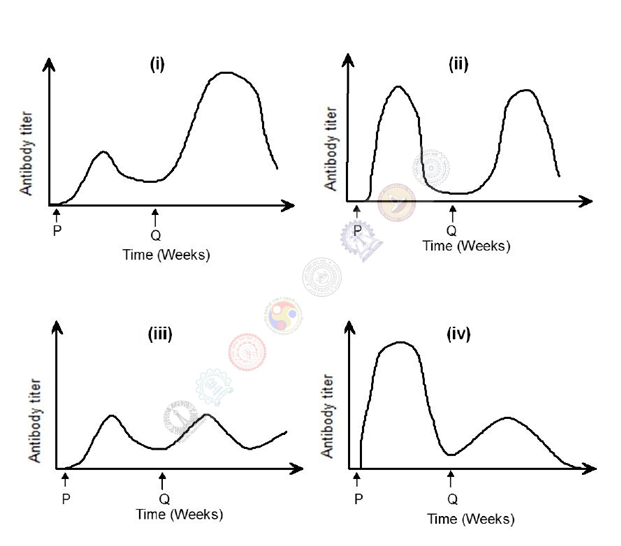
\includegraphics[width=0.8\columnwidth]{figs/fig_q66.png}
    \caption{Adaptive immune response graphs}
    \label{fig:q66}
\end{figure}

\begin{enumerate}
\begin{multicols}{2}
\item (i)
\item (ii)
\item (iii)
\item (iv)
\end{multicols}
\end{enumerate}


\item A bactericidal agent X is added after 3 hours of growth of a bacterial culture. Following the addition of X, the bacterial growth was measured using the standard plate count method till 24 hours. Which one of the following figures is the most accurate representation of the action of X?\hfill $\brak{\text{GATE XL 2017}}$

\begin{figure}[H]
    \centering
    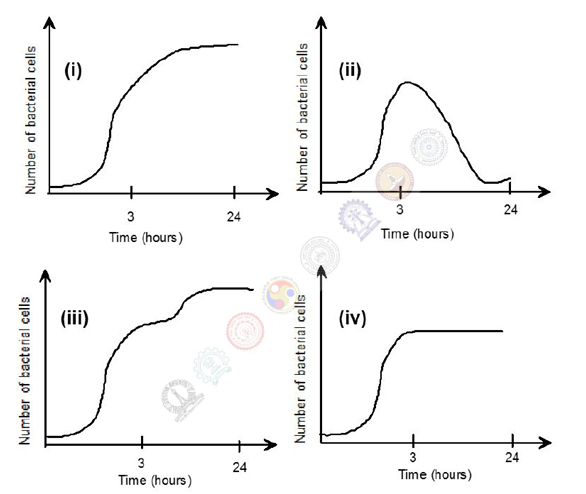
\includegraphics[width=0.8\columnwidth]{figs/fig_q67.png}
    \caption{Action of bactericidal agent X}
    \label{fig:q67}
\end{figure}

\begin{enumerate}
\begin{multicols}{2}
\item (i)
\item (ii)
\item (iii)
\item (iv)
\end{multicols}
\end{enumerate}


\item Match the diseases given in \textbf{Group I} with their causative agents from \textbf{Group II}.  \hfill $\brak{\text{GATE XL 2017}}$

\begin{multicols}{2}
\noindent \textbf{Group I} \\
P) Plague \\
Q) Rabies \\
R) Q fever \\
S) Malaria \\

\columnbreak

\noindent \textbf{Group II} \\
I. \textit{Coxiella burnetii} \\
II. \textit{Plasmodium} spp. \\
III. \textit{Yersinia pestis} \\
IV. \textit{Lyssavirus} \\
\end{multicols}

\begin{enumerate}
\begin{multicols}{2}
\item P-III, Q-IV, R-I, S-II
\item P-III, Q-I, R-II, S-IV
\item P-II, Q-III, R-I, S-II
\item P-III, Q-I, R-IV, S-II
\end{multicols}
\end{enumerate}


\clearpage
\item Match the enzymes given in \textbf{Group I} with the events from \textbf{Group II}. \hfill $\brak{\text{GATE XL 2017}}$ 

\begin{multicols}{2}
\noindent \textbf{Group I} \\
P) UvrABC endonuclease \\
Q) Reverse transcriptase \\
R) AP endonuclease \\
S) ATP sulfurylase \\

\columnbreak

\noindent \textbf{Group II} \\
I. Retrovirus replication \\
II. Base excision repair \\
III. Nucleotide excision repair \\
IV. Pyrosequencing \\
\end{multicols}

\begin{enumerate}
\begin{multicols}{2}
\item P-II, Q-I, R-IV, S-III
\item P-III, Q-I, R-II, S-IV
\item P-IV, Q-III, R-I, S-II
\item P-II, Q-I, R-III, S-IV
\end{multicols}
\end{enumerate}

\item Match the terms given in \textbf{Group I} with the descriptions from \textbf{Group II}.  \hfill $\brak{\text{GATE XL 2017}}$

\begin{multicols}{2}
\noindent \textbf{Group I} \\
P) Photoautotrophs \\
Q) Chemoautotrophs \\
R) Photoheterotrophs \\
S) Chemoheterotrophs \\

\columnbreak

\noindent \textbf{Group II} \\
I. Use inorganic chemical reactions for energy production \\
II. Use organic compounds for energy production \\
III. Use sunlight as energy source and carbon dioxide as carbon source \\
IV. Use sunlight as energy source and organic compounds as carbon source \\
\end{multicols}

\begin{enumerate}
\begin{multicols}{2}
\item P-III, Q-I, R-IV, S-II
\item P-III, Q-I, R-II, S-IV
\item P-IV, Q-III, R-I, S-II
\item P-II, Q-IV, R-III, S-I
\end{multicols}
\end{enumerate}

\item One-ml sample of a bacterial culture was serially diluted to 10$^5$ times, and 46 colonies were obtained after plating this diluted sample on an agar medium. The number of cells present per ml in the undiluted original sample were \underline{\rule{2cm}{0pt}} \hfill $\brak{\text{GATE XL 2017}}$


\item The transformation efficiency of competent cells prepared in a laboratory is 10$^4$ CFU/$\mu$g of plasmid DNA. If 0.01 $\mu$g of this plasmid is used to transform these competent cells, the number of transformed bacteria in CFU after plating will be \underline{\rule{2cm}{0pt}} \hfill $\brak{\text{GATE XL 2017}}$


\item Assume that the average DNA content of a single microbial cell is 4 femtogram. A soil sample analyzed for its microbial community DNA is found to contain 0.32 $\mu$g DNA per gram of the soil. The number of microbial cells per milligram of the soil are \underline{\rule{2cm}{0pt}} \hfill $\brak{\text{GATE XL 2017}}$


\item Assume that a bacterial culture has a mean generation time of 2 hours. If the number of bacteria present after 24 hours of culture are 4.1 $\times$ 10$^7$, the initial number of bacteria present were \underline{\rule{2cm}{0pt}} \hfill $\brak{\text{GATE XL 2017}}$


\item The minimal inhibitory concentration (MIC) of an antibiotic X against \textit{Clostridium tetani}, \textit{Staphylococcus} sp., \textit{Shigella} sp., and \textit{Streptococcus} sp. is 25, 15, 2 and 1 $\mu$g/ml, respectively. Assuming that the bioavailable concentration of X in an animal model is 20 $\mu$g/ml, which one of these bacteria may develop resistance against X in the animal model?\hfill $\brak{\text{GATE XL 2017}}$

\begin{enumerate}
\begin{multicols}{2}
\item \textit{Clostridium tetani}
\item \textit{Staphylococcus} sp.
\item \textit{Shigella} sp.
\item \textit{Streptococcus} sp.
\end{multicols}
\end{enumerate}

\section*{Zoology (XL-T)}

\setcounter{enumi}{75}

\item The characteristic feature of deuterostomes is depicted by \hfill $\brak{\text{GATE XL 2017}}$
\begin{enumerate}
    \item coelom formed by the hollowing out of a previously solid cord of mesodermal cells
    \item spiral and determinate cleavage
    \item formation of mouth from blastopore
    \item formation of anus from blastopore
\end{enumerate}

\item One of the most remarkable features of evolution is the formation of amnion and allantois. This appeared for the ``first time'' in evolutionary time scale in \hfill $\brak{\text{GATE XL 2017}}$
\begin{enumerate}
\begin{multicols}{2}
    \item reptiles
    \item birds
    \item fishes
    \item humans
\end{multicols}
\end{enumerate}

\item A woman with blood group A gave birth to a baby with blood group AB. The blood group of the father would be \hfill $\brak{\text{GATE XL 2017}}$
\begin{enumerate}
\begin{multicols}{2}
    \item only AB
    \item only B
    \item either AB or B
    \item blood group O
\end{multicols}
\end{enumerate}

\item The enzyme amylase can break alpha glycosidic linkages between glucose monomers. Hence, amylase can digest which one of the following carbohydrates? \hfill $\brak{\text{GATE XL 2017}}$
\begin{enumerate}
\begin{multicols}{2}
    \item Cellulose
    \item Starch
    \item Chitin
    \item Xylans
\end{multicols}
\end{enumerate}

\item The metabolic pathway which is common to both fermentation and cellular respiration is \hfill $\brak{\text{GATE XL 2017}}$
\begin{enumerate}
\begin{multicols}{2}
    \item the TCA cycle
    \item the electron transport chain
    \item glycolysis
    \item synthesis of acetyl CoA from pyruvate
\end{multicols}
\end{enumerate}

\item A female ``Spotted sand piper'' courts males repeatedly. This behavior can be explained by the term \hfill $\brak{\text{GATE XL 2017}}$
\begin{enumerate}
\begin{multicols}{2}
    \item polyandry
    \item polygyny
    \item monogamy
    \item sexual cannibalism
\end{multicols}
\end{enumerate}

\item Malaria is caused by \textit{Plasmodium} species, which is a parasite having a complex life cycle. The fusion between male and female gametocytes of \textit{Plasmodium} happens inside \hfill $\brak{\text{GATE XL 2017}}$
\begin{enumerate}
\begin{multicols}{2}
    \item human liver
    \item human RBCs
    \item mosquito midgut
    \item mosquito salivary glands
\end{multicols}
\end{enumerate}

\item Aromatase inhibitors are often prescribed for post-menopausal women to treat estrogen receptor positive breast cancer patients, because these class of drugs \hfill $\brak{\text{GATE XL 2017}}$
\begin{enumerate}
    \item reduce prostaglandin biosynthesis
    \item reduce the level of estradiol biosynthesis
    \item inhibit conversion of testosterone to dihydrotestosterone
    \item are non-toxic in post-menopausal women
\end{enumerate}

\item The covalent modification performed by kinases which regulate proteins in signaling pathways is \hfill $\brak{\text{GATE XL 2017}}$
\begin{enumerate}
\begin{multicols}{2}
    \item glycosylation
    \item methylation
    \item ubiquitination
    \item phosphorylation
\end{multicols}
\end{enumerate}

\item Which one of the following statements is NOT correct? \hfill $\brak{\text{GATE XL 2017}}$
\begin{enumerate}
    \item During metaphase, the 2 copies of chromosomal DNA are held together at the centromere
    \item The short arm of chromosomes is referred to as p and the long arm is referred to as q
    \item The terminal structures at the end of the chromatids are referred to as telomeres
    \item The terms heterochromatin and euchromatin refer to the active and repressed regions of the chromosome respectively
\end{enumerate}

\item A particular species is found to have 2n=16 chromosomes. The number of linkage groups in this species will be \underline{\rule{2cm}{0pt}} \hfill $\brak{\text{GATE XL 2017}}$

\item In the Meselson and Stahl experiment, \textit{E. coli} was grown in a medium containing $^{15}$NH$_4$Cl. After 24 hours, \textit{E. coli} were transferred to medium containing $^{14}$NH$_4$Cl. After the fourth generation in medium containing $^{14}$NH$_4$Cl, the ratio between hybrids ($^{15}$N/$^{14}$N) and light ($^{14}$N/$^{14}$N) labeled DNA will be $1:n$, where the value of $n$ is \underline{\rule{2cm}{0pt}} \hfill $\brak{\text{GATE XL 2017}}$

\item The population data present in an island is as follows \hfill $\brak{\text{GATE XL 2017}}$

\begin{align*}
\text{Genotype} & \quad \text{Number}\\
AA & \quad 300\\
Aa & \quad 500\\
aa & \quad 200\\
\text{Total} & \quad 1000
\end{align*}

The allele frequency of $A$ (upto two decimals) will be \underline{\rule{2cm}{0pt}}

\item A cell in G1 phase has 16 chromosomes. The total number of chromatids that would be found per cell during Metaphase II of meiosis are \underline{\rule{2cm}{0pt}} \hfill $\brak{\text{GATE XL 2017}}$

\item Upon activation of phospholipase C by ligand binding to G-protein coupled receptor, the Ca$^{2+}$ concentration in cytosol will \hfill $\brak{\text{GATE XL 2017}}$
\begin{enumerate}
    \item decrease due to blockage of InsP$_3$ gated channel on endoplasmic reticulum
    \item decrease due to blockage of InsP$_3$ gated channel on plasma membrane
    \item increase due to efflux of Ca$^{2+}$ from InsP$_3$ gated channel on mitochondria
    \item increase due to efflux of Ca$^{2+}$ from InsP$_3$ gated channel on endoplasmic reticulum as well as influx of Ca$^{2+}$ from InsP$_3$ gated channel on plasma membrane
\end{enumerate}

\item Match the molecules in \textbf{Group I} with their function in \textbf{Group II}. \hfill $\brak{\text{GATE XL 2017}}$

\begin{multicols}{2}
\noindent \textbf{Group I} \\
P) Transferrin \\
Q) Insulin \\
R) $\alpha$-macroglobulin \\
S) Fibronectin \\

\columnbreak

\noindent \textbf{Group II} \\
I. Uptake of glucose \\
II. Binds iron \\
III. Substratum for cell attachment \\
IV. Proteinase inhibitor \\
V. Binds to oxygen in RBC \\
\end{multicols}

\begin{enumerate}
\begin{multicols}{2}
\item P-III, Q-I, R-IV, S-III
\item P-II, Q-I, R-V, S-III
\item P-II, Q-I, R-IV, S-II
\item P-I, Q-III, R-II, S-V
\end{multicols}
\end{enumerate}

\item If a heavy chain of an antibody molecule weighs 65,000 Daltons (Da) and a light chain weighs 25,000 Da, the approximate calculated weight of an IgM antibody in Da will be \hfill $\brak{\text{GATE XL 2017}}$
\begin{enumerate}
\begin{multicols}{2}
    \item 90,000
    \item 180,000
    \item 360,000
    \item 900,000
\end{multicols}
\end{enumerate}
\clearpage
\item Match the signaling pathways in \textbf{Group I} with their functions in \textbf{Group II}, during the process of development. \hfill $\brak{\text{GATE XL 2017}}$

\begin{multicols}{2}
\noindent \textbf{Group I} \\
P) Hedgehog signaling \\
Q) Hox proteins \\
R) Wnt signaling \\
S) Notch signaling \\

\columnbreak

\noindent \textbf{Group II} \\
I. Involved in signaling at 4-cell embryo stage in \textit{C. elegans} through glp 1 expression \\
II. Involves frizzled receptor on target cell membrane and establish polarity in insects \\
III. Plays critical role in facial morphogenesis in vertebrates and its mutation causes cyclopia \\
IV. Required for T-bx transcription factor expression for vertebrate limb development \\
\end{multicols}

\begin{enumerate}
\begin{multicols}{2}
\item P-III, Q-II, R-IV, S-I
\item P-III, Q-IV, R-II, S-I
\item P-IV, Q-II, R-II, S-III
\item P-II, Q-IV, R-I, S-II
\end{multicols}
\end{enumerate}

\item In a population which is in Hardy-Weinberg equilibrium, the frequency of the recessive genotype of a certain trait is 0.09. The percentage of individuals with heterozygous genotype is \underline{\rule{2cm}{0pt}}\% \hfill $\brak{\text{GATE XL 2017}}$

\item An enzyme preparation has activity of 2 Units per 20 $\mu$l, and protein concentration 0.4 mg/ml. The specific activity (Units/mg) of this enzyme will be \underline{\rule{2cm}{0pt}} \hfill $\brak{\text{GATE XL 2017}}$

\section*{Food Technology (XL-U)}
\setcounter{enumi}{95}

\item Indicate the correct group that contains a monosaccharide, a disaccharide and a trisaccharide. \hfill \brak{\text{GATE XL 2017}}
\begin{enumerate}
\begin{multicols}{2}
    \item Glucose, sucrose, mannose
    \item Ribose, lactose, raffinose
    \item Mannose, maltose, lactose
    \item Raffinose, stachyose, glucose
\end{multicols}
\end{enumerate}

\item In which of the following products, `must' is used as the substrate for fermentation? \hfill \brak{\text{GATE XL 2017}}
\begin{enumerate}
\begin{multicols}{2}
    \item Beer
    \item Wine
    \item Idli
    \item Tempeh
\end{multicols}
\end{enumerate}

\item Identify the foodborne illness which is not caused by bacteria. \hfill \brak{\text{GATE XL 2017}}
\begin{enumerate}
\begin{multicols}{2}
    \item Botulism
    \item Listeriosis
    \item Vibriosis
    \item Cysticercosis
\end{multicols}
\end{enumerate}

\item Nutrient composition of wheat flour changes with extent of extraction from whole wheat grain. Which of the following statements is true if the extraction rate increased from 50\% to 90\%? \hfill \brak{\text{GATE XL 2017}}
\begin{enumerate}
    \item Starch increases, protein increases, fat increases, mineral increases
    \item Starch decreases, protein increases, fat increases, mineral increases
    \item Starch decreases, protein decreases, fat increases, mineral decreases
    \item Starch decreases, protein increases, fat decreases, mineral decreases
\end{enumerate}

\item You have two samples of milk, one (X) with 3.8\% fat and another (Y) with 0.5\% fat. In order to produce a milk with 3.5\% fat, 100 ml of Y should be mixed with \underline{\rule{2cm}{0pt}} ml of X. \hfill \brak{\text{GATE XL 2017}}

\item Match the items in Column I with the items in Column II in relation to food safety and standards. \hfill \brak{\text{GATE XL 2017}}

\begin{multicols}{2}
\noindent \textbf{Column I} \\
P) HACCP \\
Q) FSSAI \\
R) CIP \\
S) CODEX \\

\columnbreak

\noindent \textbf{Column II} \\
1. International food standards \\
2. Quality control protocol \\
3. Food plant sanitation and hygiene protocol \\
4. Indian food standards \\
\end{multicols}

\begin{enumerate}
\begin{multicols}{2}
    \item P-2, Q-4, R-3, S-1
    \item P-4, Q-3, R-2, S-1
    \item P-1, Q-4, R-2, S-3
    \item P-4, Q-2, R-3, S-1
\end{multicols}
\end{enumerate}

\item A 50\% sucrose solution at 20\degree C is flowing at a rate of 3.5 m$^3$/h through a pipe with an inside diameter of 0.0475 m and length of 12 m. The viscosity and the density of the solution are 15.43 cp and 1232 kg/m$^3$, respectively. The Reynolds number of the flow is \underline{\rule{2cm}{0pt}}. \hfill \brak{\text{GATE XL 2017}}

\item In a pineapple juice, fibre particles having mean diameter of 160 $\mu$m and density of 1075 kg/m$^3$ are settling by gravity. If the density and viscosity of the juice are 1015 kg/m$^3$ and 0.98 cp, respectively, terminal velocity of the fibre particles is \underline{\rule{2cm}{0pt}} mm/s. \hfill \brak{\text{GATE XL 2017}}

\item Power consumption in liquid mixing is proportional to \underline{\rule{2cm}{0pt}}. \hfill \brak{\text{GATE XL 2017}}
\begin{enumerate}
    \item Power number $\times$ liquid density $\times$ (rotational speed)$^3 \times$ (impeller diameter)$^5$
    \item Power number $\times$ liquid density $\times$ (rotational speed)$^2 \times$ (impeller diameter)$^3$
    \item Liquid density $\times$ viscosity of the liquid $\times$ (rotational speed)$^2 \times$ (impeller diameter)$^3$
    \item Acceleration due to gravity $\times$ liquid density $\times$ (rotational speed)$^3 \times$ (impeller diameter)$^5$
\end{enumerate}

\item In dye-reduction test for estimation of viable microorganisms, the most commonly used dyes are methylene blue, triphenyltetrazolium-chloride and \underline{\rule{2cm}{0pt}}. \hfill \brak{\text{GATE XL 2017}}
\begin{enumerate}
\begin{multicols}{2}
    \item Malachite green
    \item Amaranth
    \item Tartrazine
    \item Resazurin
\end{multicols}
\end{enumerate}

\item Match the following items of \textbf{Group I} with the items of \textbf{Group II} in relation to the quality of fat. \hfill $\brak{\text{GATE XL 2017}}$

\begin{multicols}{2}
\noindent \textbf{Group I} \\
P) Saponification number \\
Q) Iodine number \\
R) Reichert Meissl number \\
S) Acetyl value \\

\columnbreak

\noindent \textbf{Group II} \\
1. Unsaturation of fatty acid \\
2. Volatile water soluble fatty acid \\
3. Hydroxy fatty acid \\
4. Molecular weight of fatty acid \\
\end{multicols}

\begin{enumerate}
\begin{multicols}{2}
\item P-1, Q-2, R-3, S-4
\item P-1, Q-3, R-4, S-2
\item P-4, Q-1, R-2, S-3
\item P-2, Q-1, R-3, S-4
\end{multicols}
\end{enumerate}

\item Match the following metabolic product (\textbf{Column I}) that indicates the quality of food (\textbf{Column II}). \hfill $\brak{\text{GATE XL 2017}}$

\begin{multicols}{2}
\noindent \textbf{Column I} \\
P) Ethanol \\
Q) Lactic acid \\
R) Trimethylamine \\
S) Volatile fatty acid \\

\columnbreak

\noindent \textbf{Column II} \\
1. Canned vegetable \\
2. Fish \\
3. Butter \\
4. Apple juice \\
\end{multicols}

\begin{enumerate}
\begin{multicols}{2}
\item P-3, Q-2, R-4, S-1
\item P-4, Q-1, R-2, S-3
\item P-4, Q-3, R-2, S-1
\item P-3, Q-4, R-2, S-1
\end{multicols}
\end{enumerate}

\item Correlate the vitamins in \textbf{Column I} with their role in promoting reaction/process in \textbf{Column II}. \hfill $\brak{\text{GATE XL 2017}}$

\begin{multicols}{2}
\noindent \textbf{Column I} \\
P) Riboflavin \\
Q) Vitamin D \\
R) Pantothenic acid \\
S) Vitamin A \\

\columnbreak

\noindent \textbf{Column II} \\
1. Visual cycle \\
2. Acyl group transfer \\
3. Regulation of Ca$^{2+}$ metabolism \\
4. Oxidation-reduction reaction \\
\end{multicols}

\begin{enumerate}
\begin{multicols}{2}
\item P-1, Q-2, R-4, S-3
\item P-2, Q-1, R-3, S-4
\item P-3, Q-4, R-1, S-2
\item P-4, Q-3, R-2, S-1
\end{multicols}
\end{enumerate}

\item A pure strain with generation time of 60 min is used in a fermentation process. Following inoculation (0 h), the strain takes 2 h for adaptation, 10 h to achieve maximum growth and 12 h to arrive at the point where the death rate is higher than the growth rate. If the inoculation load is 100 cells, the total population at the end of 10 h will be \underline{\rule{2cm}{0pt}}. \hfill $\brak{\text{GATE XL 2017}}$

\item Refer to the shear stress-shear rate plot shown in Fig. 10. Match the lines \textbf{Column I} with appropriate rheological behavior \textbf{Column II}. \hfill $\brak{\text{GATE XL 2017}}$

\begin{figure}[H]
\centering
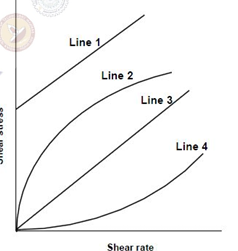
\includegraphics[width=0.5\columnwidth]{figs/fig_110.png}
\caption{\centering Shear stress-shear rate plot with Lines 1-4}
\label{fig:placeholder_110}
\end{figure}

\begin{multicols}{2}
\noindent \textbf{Column I} \\
P) Line 1 \\
Q) Line 2 \\
R) Line 3 \\
S) Line 4 \\

\columnbreak

\noindent \textbf{Column II} \\
1. Dilatant \\
2. Newtonian \\
3. Pseudoplastic \\
4. Bingham plastic \\
\end{multicols}

\begin{enumerate}
\begin{multicols}{2}
\item P-2, Q-3, R-4, S-1
\item P-1, Q-3, R-4, S-2
\item P-2, Q-4, R-3, S-1
\item P-4, Q-3, R-2, S-1
\end{multicols}
\end{enumerate}

\item Water flowing at a rate of 1 kg/min is heated from 12 to 80 \degree C with flue gas supplied at a rate of 3 kg/min. The temperature and specific heat of the flue gas are 180 \degree C and 1.05 kJ/kg.K, respectively. If specific heat of water is 4.2 kJ/kg.K and the flow is parallel, then the logarithmic mean temperature difference will be \underline{\rule{2cm}{0pt}} \degree C. \hfill $\brak{\text{GATE XL 2017}}$

\item The Lineweaver-Burk plot of an enzymatic reaction shows $V_{\max}$ of 160 $\mu$mol/l.min and $K_m$ of 60 $\mu$mol/l. For a substrate concentration of 40 $\mu$mol/l, the velocity of the reaction is estimated to be \underline{\rule{2cm}{0pt}} $\mu$mol/l.min. \hfill $\brak{\text{GATE XL 2017}}$

\item A suspension containing $2\times10^{4}$ spores of organism A having a $D_{121.1^{\circ}\text{C}}$ value of 1.5 min and $8\times10^{5}$ spores of organism B having a $D_{121.1^{\circ}\text{C}}$ value of 0.8 min is heated at a constant temperature of 121.1 \degree C. The heating time needed to obtain a probability of spoilage ``1 in 1000'' is \underline{\rule{2cm}{0pt}} min. \hfill $\brak{\text{GATE XL 2017}}$

\item In an evaporation process, a compressor picks up 0.05 m$^{3}$ air in each revolution and compresses 500 kg of air per minute. If the specific volume of air is 0.9 m$^{3}$/kg, then the compressor speed is \underline{\rule{2cm}{0pt}} rpm. \hfill $\brak{\text{GATE XL 2017}}$

\item For a soybean oil extraction system, solvent:soy ratio is maintained at 0.5:1 (w/w). Original seed contains 18\% oil (w/w). If the meal (soy solid) after final desolventization has 0.01 kg oil per kg \emph{oil-free} meal, then the effectiveness of the solvent (kg oil/kg solvent) in the extraction process is \underline{\rule{2cm}{0pt}}. \hfill $\brak{\text{GATE XL 2017}}$

\item The event would have been successful if you \underline{\rule{2cm}{0pt}} able to come. \hfill $\brak{\text{GATE XL 2017}}$
\begin{enumerate}
\begin{multicols}{2}
    \item are
    \item had been
    \item have been
    \item would have been
\end{multicols}
\end{enumerate}

\item There was no doubt that their work was \underline{thorough}. Which of the words below is closest in meaning to the underlined word above? \hfill $\brak{\text{GATE XL 2017}}$
\begin{enumerate}
\begin{multicols}{2}
    \item pretty
    \item complete
    \item sloppy
    \item haphazard
\end{multicols}
\end{enumerate}

\item Four cards lie on a table. Each card has a number printed on one side and a colour on the other. The faces visible on the cards are 2, 3, red, and blue. Proposition: If a card has an even value on one side, then its opposite face is red. The cards which MUST be turned over to verify the above proposition are \hfill $\brak{\text{GATE XL 2017}}$
\begin{enumerate}
\begin{multicols}{2}
    \item 2, red
    \item 2, 3, red
    \item 2, blue
    \item 2, red, blue
\end{multicols}
\end{enumerate}

\item What is the value of $x$ when $81\times\brak{\dfrac{16}{25}}^{x+2}\div\brak{\dfrac{3}{5}}^{2x+4}=144\,$? \hfill $\brak{\text{GATE XL 2017}}$
\begin{enumerate}
\begin{multicols}{2}
    \item 1
    \item $-1$
    \item 2
    \item Cannot be determined
\end{multicols}
\end{enumerate}

\item Two dice are thrown simultaneously. The probability that the product of the numbers appearing on the top faces of the dice is a perfect square is \hfill $\brak{\text{GATE XL 2017}}$
\begin{enumerate}
\begin{multicols}{2}
    \item $1/9$
    \item $2/9$
    \item $1/3$
    \item $4/9$
\end{multicols}
\end{enumerate}

\item Bhaichung was observing the pattern of people entering and leaving a car service centre. There was a single window where customers were being served. He saw that people inevitably came out of the centre in the order that they went in. However, the time they spent inside seemed to vary a lot: some people came out in a matter of minutes while for others it took much longer. From this, what can one conclude? \hfill $\brak{\text{GATE XL 2017}}$
\begin{enumerate}
    \item The centre operates on a first-come-first-served basis, but with variable service times, depending on specific customer needs
    \item Customers were served in an arbitrary order, since they took varying amounts of time for service completion in the centre
    \item Since some people came out within a few minutes of entering the centre, the system is likely to operate on a last-come-first-served basis
    \item Entering the centre early ensured that one would have shorter service times and most people attempted to do this
\end{enumerate}

\item A map shows the elevations of Darjeeling, Gangtok, Kalimpong, Pelling, and Siliguri. Kalimpong is at a lower elevation than Gangtok. Pelling is at a lower elevation than Gangtok. Pelling is at a higher elevation than Siliguri. Darjeeling is at a higher elevation than Gangtok. Which of the following statements can be inferred from the paragraph above? \hfill $\brak{\text{GATE XL 2017}}$

\begin{align*}
\text{i. } & \text{Pelling is at a higher elevation than Kalimpong}\\
\text{ii. } & \text{Kalimpong is at a lower elevation than Darjeeling}\\
\text{iii. } & \text{Kalimpong is at a higher elevation than Siliguri}\\
\text{iv. } & \text{Siliguri is at a lower elevation than Gangtok}
\end{align*}

\begin{enumerate}
\begin{multicols}{2}
    \item Only ii
    \item Only ii and iii
    \item Only iii and iv
    \item Only iii and iv
\end{multicols}
\end{enumerate}

\item $P, Q, R, S, T$ and $U$ are seated around a circular table. $R$ is seated two places to the right of $Q$. $P$ is seated three places to the left of $R$. $S$ is seated opposite $U$. If $P$ and $U$ now switch seats, which of the following must necessarily be true? \hfill $\brak{\text{GATE XL 2017}}$
\begin{enumerate}
    \item $P$ is immediately to the right of $R$
    \item $T$ is immediately to the left of $P$
    \item $T$ is immediately to the left of $P$ or $P$ is immediately to the right of $Q$
    \item $U$ is immediately to the right of $R$ or $P$ is immediately to the left of $T$
\end{enumerate}

\item Budhan covers a distance of 19 km in 2 hours by cycling one fourth of the time and walking the rest. The next day he cycles (at the same speed as before) for half the time and walks the rest (at the same speed as before) and covers 26 km in 2 hours. The speed in km/h at which Budhan walks is \hfill $\brak{\text{GATE XL 2017}}$
\begin{enumerate}
\begin{multicols}{2}
    \item 1
    \item 4
    \item 5
    \item 6
\end{multicols}
\end{enumerate}

\item The points in the graph below represent the halts of a lift for durations of 1 minute, over a period of 1 hour. \hfill $\brak{\text{GATE XL 2017}}$

\begin{figure}[H]
\centering
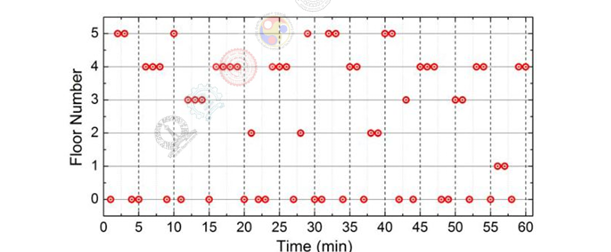
\includegraphics[width=0.75\columnwidth]{figs/fig_125.png}
\caption{\centering Lift halts over time}
\label{fig:placeholder_125}
\end{figure}

Which of the following statements are correct?

\begin{align*}
\text{i. } & \text{The elevator never moves directly from any non-ground floor to another non-ground floor over the one hour period}\\
\text{ii. } & \text{The elevator stays on the fourth floor for the longest duration over the one hour period}
\end{align*}

\begin{enumerate}
\begin{multicols}{2}
    \item Only i
    \item Only ii
    \item Both i and ii
    \item Neither i nor ii
\end{multicols}
\end{enumerate}

\end{enumerate}
\end{document}
